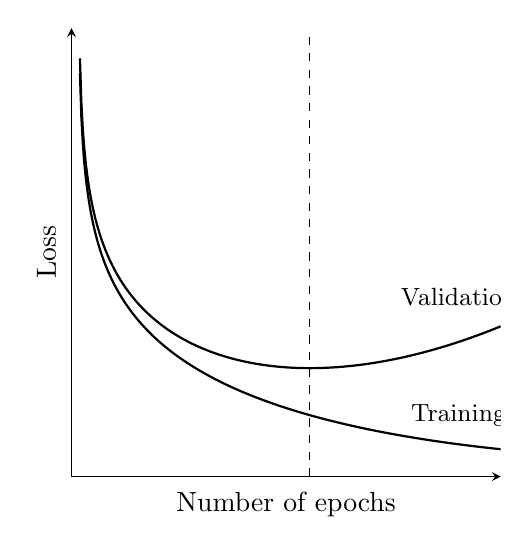
\begin{tikzpicture}
	\begin{axis}[
		xlabel=Number of epochs,
		ylabel=Loss,
		width=0.58\textwidth,
        height=\axisdefaultheight,
        axis x line=bottom,
        axis y line=left,
        % axis lines*=left,
        ymin=-0.1,
        ymax=3,
        xmin=-0.05,
        xmax=3,
        xtick=\empty,
	    ytick=\empty,
	]

	\addplot[samples=300, domain=0:3, thick, black]   {-(1 - x / 5) * log10(x / 5)};
	\addplot[samples=300, domain=0:3, thick, black]    {-(1 - x / 5) * log10(x / 5) + (x^2) / 12 + 0.1};

	\node[] at (2.7, 1.14) {\small{Validation}};
	\node[] at (2.7, 0.32) {\small{Training}};
	\draw[dashed] (1.64, -0.1) -- (1.64, 3);
	\end{axis}
\end{tikzpicture}